\documentclass[11pt]{report}
\usepackage{graphicx}
\usepackage{amsmath}
\usepackage{amsthm}
\usepackage[spanish]{babel}

\newtheorem{example}{Ejemplo}[section]

\title{Máquinas y Comandos Eléctricos}
\author{Joaquín Gómez --- 5to ``A''}
\date{2025}

\begin{document}
\maketitle

\chapter{Autotransformadores}
Los autotransformadores poseen una parte del devanado en común, que corresponde tanto al 
primario como al secundario. 
El principio de funcionamiento es el mismo que el del transformador común, entonces la relación de 
transformación entre las tensiones, las intensidades de corriente y el número de vueltas se mantienen.

Las corrientes primarias y secundarias están en oposición y la corriente total que circula por las espiras
en común es igual a la diferencia de la corriente del devanado de baja tensión y el devanado de alta tensión
\begin{equation}
    I_c = I_{AT} - I_{BT} \quad \textnormal{si } V_{AT} > V_{BT}   
\end{equation}
Para que un autotransformador funcione adecuadamente, los devanados deben tener el mismo sentido de bobinado.

\section{Autotransformadores Reductores}
Si se aplica una tensión alterna entre los puntos A y B, y se mide la tensión de salida entre los puntos C y D,
se dice que el autotransformador es un reductor de tensión

\begin{figure}[h]
    \begin{center}
        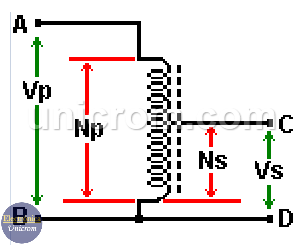
\includegraphics[width=200px]{autotransformador-reductor.png}
    \end{center}
    \caption{Autotransformador reductor}
\end{figure}

En este caso, la relación de vueltas del autotransformador es:
\begin{equation}
    \frac{N_s}{N_p} < 1 
\end{equation}

\section{Autotransformadores elevadores}
Si se aplica una tensión de alimentación alterna entre los puntos A y B, y se mide la tensión de salida entre los puntos C y D, se dice que el autotransformador es elevador de tensión.

\begin{figure}[h]
    \begin{center}
        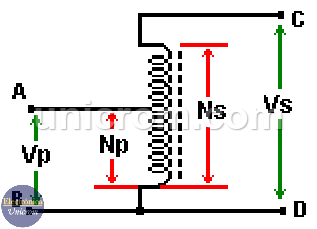
\includegraphics[width=200px]{autotransformador-elevador.png}
    \end{center}
    \caption{Autotransformador elevador}
\end{figure}

En este caso, la relación de vueltas del autotransformador es: 
\begin{equation}
    \frac{N_s}{N_p} > 1
\end{equation}

Los autotransformadores tienen la ventaja sobre los transformadores comunes 
de un peso y costo menor. En lugar de tener un bobinado de AT de $N_1$ espiras,
se debe preveer para el bobinado de BT, con un número $N_2$ de espiras, un número 
adicional de espiras de $N_1-N_2$. También hay que tener en cuenta que el conductor
de la sección común del bobinado debe tener una sección de alambre en función de la 
diferencia de corrientes entre AT y BT, o sea, $I_2-I_1$.

Otra ventaja es la de no necesitar aislamiento entre los bobinados primario y secundario.
Sin embargo, esto trae como desventaja que el bobinado primario no es independiente del 
secundario. Esto causa peligro para una persona, pues, entre tierra y el hilo común del 
secundario y el primario existe la tensión del primario (Ver figura 1).

\begin{example}
        Se requiere un autotransformador para aumentar un voltaje de $220V$ a $250V$.
        El número total de espiras que tiene el devanado principal es de $2000$. Determine 
        la posición del punto de toma primario, la corriente primaria y secundaria cuando 
        la salida tiene una potencia de $10{kVA}$. Y la economía de cobre ahorrada\footnote{La 
        relación $n$ se define como la relación entre el voltaje más bajo y el voltaje más alto,
        entonces se puede demostrar que el ahorro de cobre es: $n\cdot100\%$}.

        Tenemos que la relación ideal de vueltas debe ser 
        \begin{equation}
            \frac{V_1}{V_2} < 1
        \end{equation}
        ya que el transformador es elevador. De forma que 
        \begin{equation}
            \frac{N_1}{N_2} < 1
        \end{equation}
        Así, tenemos que idealmente 
        \begin{equation}
            \begin{split}
                \frac{V_1}{V_2} &= \frac{N_1}{N_2} \\
                \frac{220V}{250V} &= \frac{N_1}{2000esp} \\
            \end{split}
        \end{equation}
        Por lo tanto 
        \begin{equation}
            \begin{split}
                N_2 &= \frac{220 V \cdot 2000esp}{250V} \\&= 1760 esp
            \end{split}
        \end{equation}        
        El porcentaje de ahorro de cobre está dado por 
        \begin{equation}
            n\cdot 100\% = \frac{V_1}{V_2}\cdot 100\% = 88\% 
        \end{equation}
        Como condición, tenemos que $P_1 = P_2$, así, podemos deducir que 
        \begin{equation}
            \begin{split}
                V_1 I_1 &= P_1 \\
                220V I_1 &= 10000VA \\
                I_1 &\approx 45.456A
            \end{split}
        \end{equation}
        \begin{equation}
            \begin{split}
                V_2 I_2 &= P_2 \\
                250V I_2 &= 10000VA \\
                I_2 &= 40A
            \end{split}
        \end{equation}
    \end{example}

    \begin{example}
        En el siguiente autotransformador reductor indicar el sentido de la corriente ($I_c$, intensidad común) que circulará por la parte del arrollamiento que tienen en común $N_1$ y $N_2$. Fundamentar el sentido de circulación.

        Si tenemos un transformador reductor, donde $V_1 > V_2$, entonces $I_1 < I_2$. Por la ley de Kirchoff tenemos 
        \begin{equation}
            \sum_k I_s^{(k)} = \sum_k I_e^{(k)}
        \end{equation}
        es decir, la suma de las corrientes de entrada es igual a las de salida. En este caso, si $I_1 < I_2$ tendremos 
        \begin{equation}
            I_2 = I_1 + I_C
        \end{equation}
        Como la corriente $I_1$ es la entrada, tenemos que $I_2$ y $I_c$ serán corrientes de salida.
        \begin{center}
            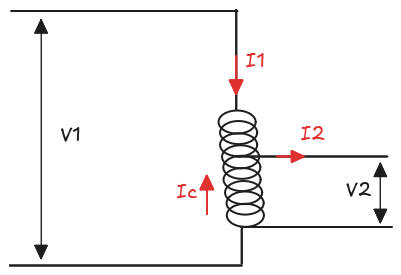
\includegraphics[width=200px]{ejemplo2.png}
        \end{center}
    \end{example}

\end{document} como
